\chapter{Aplikacijska programska sučelja}

Aplikacijska programska sučelja služe za olakšano korištenje usluga, protokola i periferija koje nudi hardver. Dostupno je mnogo API-ja za ESP32-C3 \cite{espressif}, no ovdje je napravljen osnovni pregled programskih sučelja koja koriste Bluetooth. 

\textit{ESP-IDF}, službeni radni okvir za razvoj softvera na ESP mikrokontrolerima, podržava dva radna okvira kao BLE domaćin:
\begin{itemize}
	\item \textit{Bluedroid}, koji podržava klasični Bluetooth i BLE,
	\item \textit{NimBLE}, koji podržava samo BLE.
\end{itemize}

Preporuka je koristiti \textit{Bluedroid} za aplikacije u kojima se može pojaviti potreba korištenja i klasičnog Bluetootha, dok je \textit{NimBLE} prikladniji pri korištenju isključivo BLE protokola radi manje potrošnje memorije. \cite{esp_bt_api}

\section{Bluedroid}

\textit{Bluedroid} je zadani stog koji se koristi kao Bluetooth domaćin. Ovaj radni okvir, osim BLE protokola, podržava i klasični Bluetooth, te pruža jednostavnije istovremeno korištenje oba protokola. Arhitektura \textit{Bluedroida} i njegov odnos sa BLE upravljačem prikazani su na slici \ref{fig:bluedroid_arch}.

\begin{figure}[ht]
	\centering
	\includegraphics[scale=0.4]{imgs/bluedroid\_arch}
	\caption{Dijagram \textit{Bluedroid} arhitekture}
	\label{fig:bluedroid_arch}
\end{figure}

\textit{Bluedroid} se može podijeliti na dva glavna sloja: BTC i BTU. BTC sloj služi kao sučelje aplikacijskom sloju te obrađuje zadatke vezane uz GATT profil. BTU sloj odgovoran je za interakciju sa BLE upravljačem. Pri obradi korisničkog zadatka, podzadaci vezani za Bluetooth proslijeđeni su nižim slojevima koji ih postupno obrađuju, te se prosljeđuju dalje niz hijerarhijsku strukturu. Svrha ovakvog dizajna je rasterećenje korisničkih zadataka i prosljeđivanje zadataka vezanih za Bluetooth nižim slojevima. \cite{esp32_bt}

U sklopu \textit{Bluedroid} API-ja nudi se nekoliko demo aplikacija koje demonstriraju različite značajke. U nastavku su tri demo aplikacije koje nude softver za klijentsku i poslužiteljsku stranu. 

Prvi primjer implementira GATT poslužitelja i klijenta. Na početku svakog programa izvršavaju se konfiguracijski koraci, poput definiranja parametara oglašavanja te stvaranje usluga i karakteristika. Nadalje, obrađuju se događaji čitanja i pisanja, uključujući i zahtjev za pisanje dugačke karakteristike, što rezultira fragmentacijom nadolazećih podataka u manje pakete. Klijentska strana skenira uređaje u blizini te traži usluge i karakteristike željenog poslužitelja. Kada pronađe traženi poslužitelj, uspostavlja se veza i vrši pretraga usluga. Na kraju, kada klijent pronađe određenu karakteristiku u pretraženim uslugama, dobiva njezinu vrijednost i pretplaćuje se za obavijesti o toj karakteristici. Na slici \ref{fig:gatt_diagram} prikazan je sekvencijski dijagram komunikacije GATT poslužitelja i klijenta.

\begin{figure}[ht]
	\centering
	\includegraphics[scale=0.2]{imgs/gatt\_diagram}
	\caption{Sekvencijski dijagram komunikacije GATT poslužitelja i klijenta \cite{esp_bt_api}}
	\label{fig:gatt_diagram}
\end{figure}

Ispis klijentske strane nalazi se na slici \ref{fig:gatt_client}. Slika prikazuje klijentovo skeniranje dostupnih uređaja odnosno reklamnih paketa. Pretraživanje se ponavlja sve dok ne pronađe paket, te se tada spaja sa pronađenim uređajem, što je vidljivo u prvoj polovici ispisa. Druga polovica prikazuje ažuriranje parametara povezivanja te dohvat informacija o poslužitelju. Događaj \texttt{ESP\_GATTC\_REG\_FOR\_NOTIFY\_EVT} označava da se klijent pretplaćuje na poslužiteljevu promjenu parametara. \texttt{ESP\_GATTC\_NOTIFY\_EVT} označava da je klijent dobio obavijest na koju se pretplatio. 

\begin{figure}[ht]
	\centering
	\includegraphics[scale=0.5]{imgs/gatt\_client}
	\caption{Ispis klijenta u demo aplikaciji za GATT profil}
	\label{fig:gatt_client}
\end{figure}

Iduća aplikacija također simulira vezu GATT poslužitelja i klijenta, no virtualnom serijskom vezom. U sustavima s klasičnim Bluetoothom, profil serijskog ulaza (engl. \textit{Serial Port Profile - SPP}) koristi se za oponašanje serijske veze putem bežične Bluetooth veze. Budući da BLE nema standardnu SPP uslugu, mora se posebno implementirati. U \textit{Bluedroid} okviru za SPP aplikacije koristi se UART transportni sloj, no po potrebi se može modificirati da koristi i druge serijske protokole, primjerice SPI. Svrha ovog načina komunikacije jest emulacija serijske veze, odnosno brzih i kratkih prijenosa podataka, zbog čega jednosmjerna propusnost može doseći do 1900 Kbps.

Kao i u prethodnoj aplikaciji, prikazano je spajanje klijenta na poslužitelj skeniranjem reklamnih paketa. Ispis klijentske aplikacije za virtualnu serijsku vezu prikazan je na slici \ref{fig:spp_client}. Ovdje su također ispisani dostupni atributi odnosno karakteristike koje klijent može pratiti. Kao što je ranije prikazano na slici \ref{fig:ble_profile_char}, svaka karakteristika ima pridružena svojstva. Druga polovica ispisa prikazuje događaje koji se zbivaju nad pojedinim atributima. Svakom je atributu pridružena jedinstvena oznaka (UUID) na temelju koje se zaključuje o kojem se atributu radi. Popis jedinstvenih identifikatora te što koji označava nalazi se na službenoj stranici Bluetootha. \cite{bluetooth_ofisl} 

\begin{figure}[ht]
	\centering
	\includegraphics[scale=0.5]{imgs/spp\_client}
	\caption{Ispis klijenta u demo aplikaciji za SPP profil}
	\label{fig:spp_client}
\end{figure}

Treći primjer testira propusnost između klijentske i poslužiteljske aplikacije. U optimalnim uvjetima ona može dosegnuti do 700 Mbps između dvije ESP32 pločice. U ovom primjeru klijent kontinuirano šalje podatke poslužitelju, a ispis prikazuje količinu podataka poslanu svake sekunde. Vidljivo je da su vrijednosti puno manje od idealnih 700 Mbps, te dosežu maksimalno oko 1500 bps. Ispis je prikazan na slici \ref{fig:throughput_client}.

\begin{figure}[ht]
	\centering
	\includegraphics[scale=0.6]{imgs/throughput\_client}
	\caption{Ispis klijenta u demo aplikaciji za propusnost}
	\label{fig:throughput_client}
\end{figure}

\section{NimBLE}

\textit{NimBLE} je konfigurabilan BLE stog koji pruža funkcije BLE domaćina i upravljača. \textit{ESP-IDF} podržava samo funkcionalnost domaćina, dok je temeljni upravljač isti za sve API-je. Podržava većinu značajki koje nudi \textit{NimBLE} API, uključujući BLE \textit{Mesh} koji omogućava mrežnu topologiju. \textit{NimBLE} domaćin može se izvoditi unutar dretve aplikacije ili može imati vlastitu dretvu. Ova je fleksibilnost podržana konfiguracijom samog okvira te omogućuje višedretvenost Bluetooth procesa.

Arhitektura \textit{NimBLE} stoga nalik je strukturi \textit{Bluedroid} API-ja. Budući da je podržan samo \textit{NimBLE} domaćin, ne i upravljač, postojeći upravljač nije kompatibilan sa domaćinom \textit{NimBLE} okvira. Stoga je implementiran dodatni sloj koji služi kao sučelje između domaćina i upravljača (engl. \textit{Virtual Host Controller Interface - VHCI}) specifičan za \textit{NimBLE} stog. Arhitektura je prikazana na slici \ref{fig:nimble_arch}. 

\begin{figure}[ht]
	\centering
	\includegraphics[scale=0.6]{imgs/nimble\_arch}
	\caption{Arhitektura \textit{NimBLE} stoga \cite{esp_bt_api}}
	\label{fig:nimble_arch}
\end{figure}

U nastavku je analizirana aplikacija koja koristi \textit{NimBLE} stog, ali i Wi-Fi povezivost. Primjer prikazuje paralelno izvođenje Wi-Fi i Bluetooth naredbi u modulu. Potrebno je unaprijed navesti parametre Wi-Fi mreže, odnosno ime mreže i lozinku, na koju će se sustav spojiti. Nakon inicijalizacije okvira, uređaj se spaja na Wi-Fi mrežu i šalje \textit{ping} poruke za provjeru veze. Istovremeno razvojni sustav oglašava pakete Bluetooth vezom koje klijenti mogu pročitati kako bi se povezali. Ispis aplikacije nakon uspješnog povezivanja na Wi-Fi prikazan je na slici \ref{fig:spojen}, dok se na slici \ref{fig:nespojen} nalazi ispis nakon neuspješnog spajanja na mrežu. Vidljivo je da je u oba slučaja omogućeno korištenje BLE stoga bez obzira na ostvarenu Wi-Fi vezu.

\begin{figure}[ht]
	\begin{minipage}[t]{0.4\textwidth}
		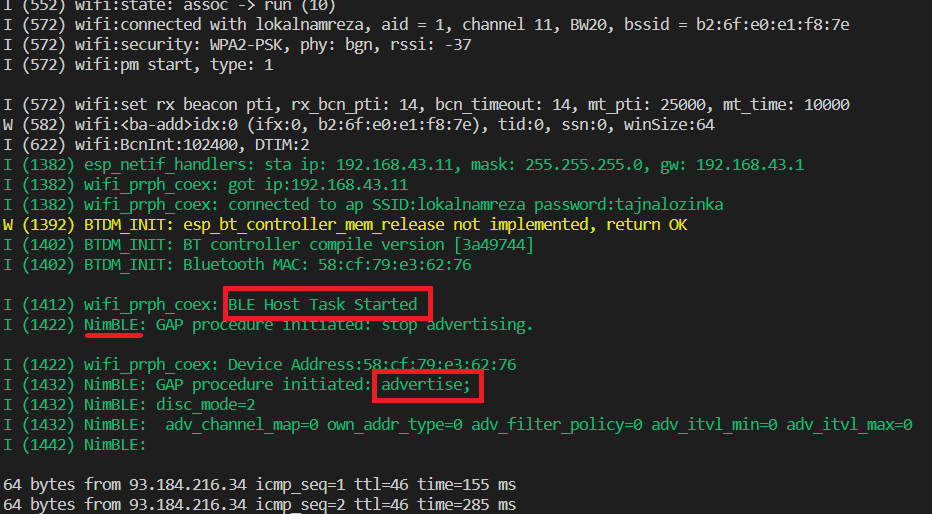
\includegraphics[width=\linewidth]{imgs/spojen}
		\caption{Ispis nakon uspješnog spajanja na Wi-Fi vezu}
		\label{fig:spojen}
	\end{minipage}
	\hspace*{\fill}
	\begin{minipage}[t]{0.4\textwidth}
		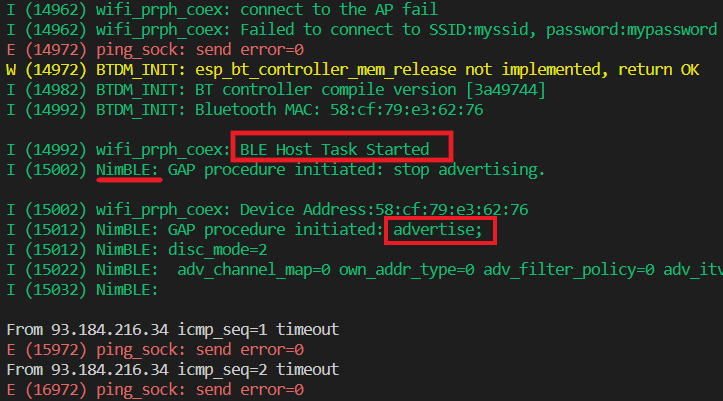
\includegraphics[width=\linewidth]{imgs/nespojen}
		\caption{Ispis nakon neuspješnog spajanja na Wi-Fi vezu}
		\label{fig:nespojen}
	\end{minipage}
\end{figure}

\subsection{BLE Mesh}

Bluetooth \textit{Mesh} umrežavanje omogućuje komunikaciju više-na-više uređaja (n:n) i optimizirano je za stvaranje mreža uređaja velikih razmjera. Uređaji mogu prenositi podatke drugim uređajima koji nisu u izravnom radijskom dometu izvornog uređaja. Na taj način isprepletene mreže mogu obuhvatiti vrlo velika fizička područja i sadržavati velik broj uređaja. Bluetooth \textit{Mesh} nije bežična komunikacijska tehnologija, već mrežna tehnologija koja ovisi o BLE protokolu. Programsko sučelje \textit{ESP-BLE-MESH} implementirano je u okviru \textit{NimBLE} radnog okvira, te podržava samo BLE protokol. 

Arhitektura \textit{ESP-BLE-MESH} sučelja sastoji se od pet ključnih dijelova:
\begin{itemize}
	\item \textit{Mesh} protokolni stog - osigurava protok mreže i razmjenu podataka,
	\item mrežno upravljanje - obavlja razne procedure za upravljanje mrežom, 
	\item značajke - dodatne mogućnosti koje sučelje nudi,
	\item sloj nositelja mreže - sloj ključan za komunikaciju s BLE stogom,
	\item aplikacije - komuniciraju s \textit{mesh} protokolnim stogom.
\end{itemize}

Sljedeći primjer koristi tri razvojna sustava ESP32-C3-DevKitM-1 i mobilni uređaj za demonstriranje mrežne topologije. Na sva tri razvojna sustava nalazi se ista poslužiteljska aplikacija koja oglašava reklamne pakete i tako omogućava spajanje mobilnog uređaja. Na mobilnom uređaju korištena je aplikacija \textit{nRF Mesh} tvrtke \textit{Nordic Semiconductors} koja omogućava mobilnom uređaju stvaranje mreže. Nakon skeniranja uređaja, u aplikaciji je moguće odabrati razvojni sustav s kojim će se uređaj spojiti. Odabirom željenog čvora aplikacija će pokušati pripojiti čvor mreži na sljedeći način:

\begin{itemize}
	\item najprije se odspaja od čvora,
	\item zatim se pokušava ponovno spojiti,
	\item nakon uspješnog spajanja uspostavlja GATT uslugu,
	\item na kraju dohvaća podatke čvora i dodaje im aplikacijski ključ koji služi za kasnije ponovno spajanje.
\end{itemize}

Na slici \ref{fig:mesh_spojen} prikazana je obavijest koja se pojavi u mobilnoj aplikaciji nakon uspješnog pripajanja čvora u mreži. U pozadini iza obavijesti moguće je vidjeti gore opisani postupak uspostave veze. Na slici \ref{fig:mesh_tri} nalazi se prikaz čvorova u mreži prikazanih u mobilnoj aplikaciji. 

\begin{figure}[ht]
	\begin{minipage}[t]{0.4\textwidth}
		\includegraphics[width=\linewidth]{imgs/mesh\_spojen}
		\caption{Obavijest u mobilnoj aplikaciji nakon spajanja čvora}
		\label{fig:mesh_spojen}
	\end{minipage}
	\hspace*{\fill}
	\begin{minipage}[t]{0.4\textwidth}
		\includegraphics[width=\linewidth]{imgs/mesh\_tri}
		\caption{Čvorovi spojeni u mrežu s mobilnim uređajem}
		\label{fig:mesh_tri}
	\end{minipage}
\end{figure}


\section{BluFi}

Iako nije namijenjen razvoju Bluetooth aplikacija, važno je istaknuti i \textit{BluFi} radni okvir. \textit{BluFi} služi za konfiguraciju Wi-Fi mreže putem Bluetooth kanala. Omogućuje siguran protokol za prijenos Wi-Fi konfiguracije na ESP32-C3. Koristeći te informacije, razvojni se sustav može spojiti na pristupnu točku ili postati pristupna točka na koju se drugi uređaji mogu spojiti.

Fragmentacija, enkripcija podataka i autentifikacija ključni su elementi okvira \textit{BluFi}. Također je moguće prilagoditi način enkripcije proizvoljnim odabirom enkripcijskih algoritama.

Povezivanje ESP32-C3 mikrokontrolera putem Bluetooth protokola na Wi-Fi mrežu odvija se na sljedeći način:
\begin{itemize}
	\item ESP32-C3 majprije mora biti postavljen u način rada kao GATT poslužitelj kako bi odašiljao reklamne podatke. 
	\item Drugi uređaj s ulogom GATT klijenta skenira reklamne pakete i povezuje se s poslužiteljem po primitku željenih paketa.
	\item Nakon uspješne GATT veze, GATT klijent šalje podatkovni okvir radi uspostave ključa za šifriranje.
	\item Nakon dogovorene enkripcijske metode i uspostavljenog ključa, klijent šalje podatkovni okvir sa podacima o Wi-Fi konfiguraciji, uključujući ime mreže i lozinku.
	\item Klijent šalje kontrolni okvir nakon čijeg se primitka poslužitelj može spojiti na Wi-Fi.
	\item Nakon spajanja, ESP32-C3 šalje kontrolni okvir s podacima o statusu Wi-Fi veze.
\end{itemize} 

Dijagram opisanog povezivanja nalazi se na slici \ref{fig:blufi_diagram}.

\begin{figure}[ht]
	\centering
	\includegraphics[scale=0.6]{imgs/blufi\_diagram}
	\caption{Sekvencijski dijagram povezivanja putem \textit{Blu-Fi} konfiguracije \cite{esp_bt_api}}
	\label{fig:blufi_diagram}
\end{figure}

Za demonstraciju mogućnosti \textit{BluFi} okvira korištena je demo aplikacija u kojoj je modul ESP32-C3 povezan na Wi-Fi pristupnu točku mobilnog uređaja. Za povezivanje je korištena mobilna aplikacija \textit{ESP BLE Prov} tvrtke \textit{Espressif} koja je namijenjena demonstraciji povezivanja razvojnog sustava s mobilnim uređajem. Korisničko sučelje aplikacije prikazano je na slici \ref{fig:mob}. Za uspostavu veze potrebno je na mobilnom uređaju omogućiti Bluetooth, lokaciju te mobilnu pristupnu točku. Nakon uspješnog povezivanja, aplikacija na razvojnom sustavu ispisat će poruku o uspješnom spajanju. Ispis se nalazi na slici \ref{fig:blufi_connect}.

\begin{figure}[ht]
	\centering
	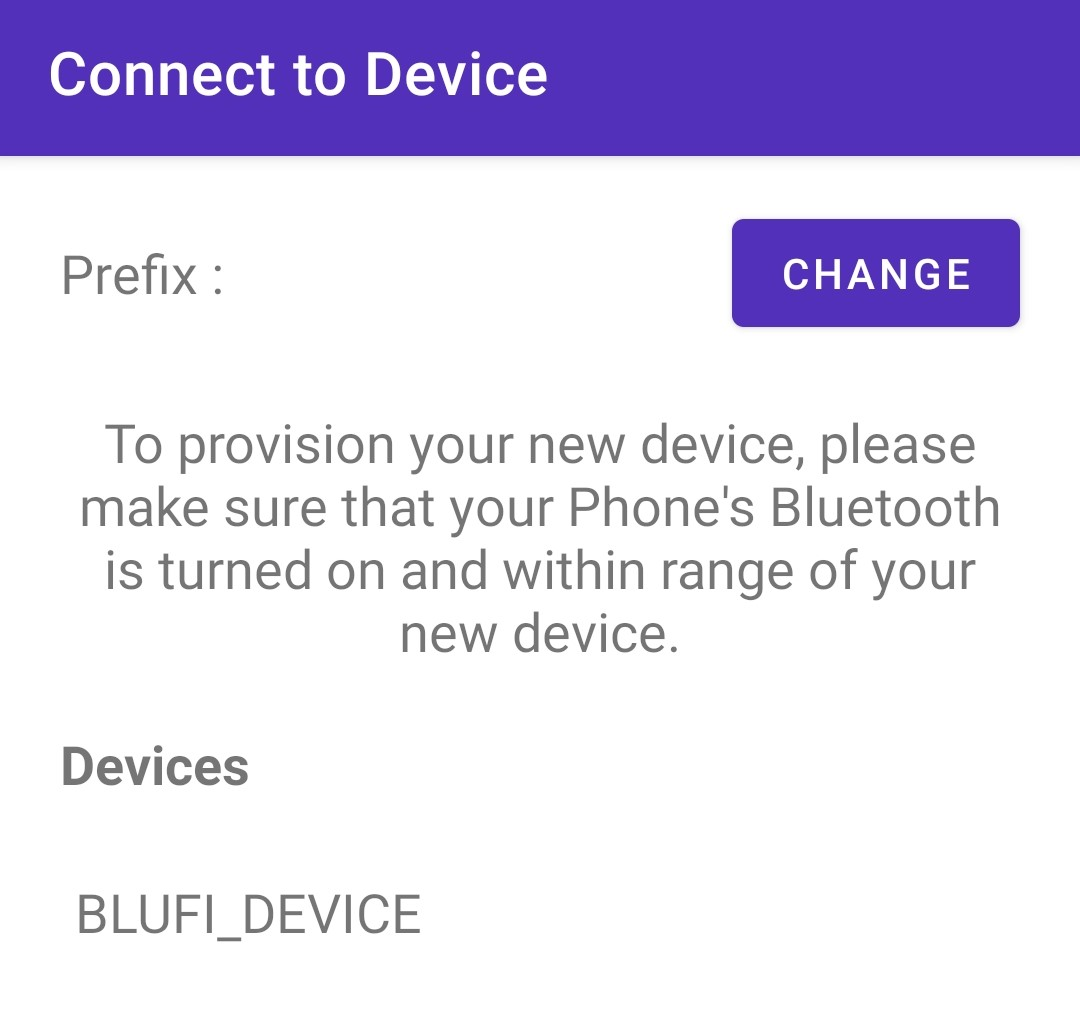
\includegraphics[scale=0.15]{imgs/mob}
	\caption{Korisničko sučelje mobilne aplikacije \textit{ESP BLE Prov}}
	\label{fig:mob}
\end{figure}


\begin{figure}[ht]
	\centering
	\includegraphics[scale=0.6]{imgs/blufi\_connect}
	\caption{Ispis demo aplikacije nakon povezivanja na Wi-Fi pristupnu točku}
	\label{fig:blufi_connect}
\end{figure}

\eject